\chapter{Affective Steering Pipeline}
\label{chap:development1_emo_steering}

This chapter demonstrates that contrastive activation addition (CAA) vectors can be constructed in the emotion context of a large language model, and that these vectors decompose naturally into a \textbf{shared emotionalisation component} and an \textbf{emotion-specific residual component}. The central empirical finding is that only the residual component is needed for reliable affective steering.

\section{Chapter Roadmap}
\label{sec:steering_roadmap_1}
This chapter proceeds through five stages that build toward that claim.

\begin{enumerate}
  \item \textbf{Prerequisites}: Before computing CAA vectors, three building blocks are required. Firstly we need a controlled dataset of emotional rewrites paired with neutral paraphrases. Then, residual-stream activations are extracted from the model, and a principled layer is selected to identify which transformer layer best abstracts pre-verbal affective structure. These are covered in Sections~\ref{sec:dataset_construction},~\ref{sec:residual_extraction}, and~\ref{sec:layer_selection}.

  \item \textbf{CAA vector construction} (Section~\ref{sec:caa_construction}): Using the extracted activations, we compute contrastive vectors for each emotion by averaging the difference between emotion-conditioned and neutral-conditioned hidden states across source texts and intensity levels.

  \item \textbf{Observation}: Inspecting the inter-emotion cosine similarities of the resulting CAA vectors reveals a striking pattern; all pairs of emotion vectors lie in the range $0.91$--$0.97$. This near-uniformity indicates that the vectors are \textbf{dominated by a shared direction activated regardless of the target emotion}, and directly motivates the decomposition introduced next.

  \item \textbf{Decomposition} (Section~\ref{sec:decomposition}): We define a shared emotionalisation vector $\mathbf{g}$ as the normalised mean of all emotion CAA vectors, and project it out by orthogonal projection to obtain emotion-specific residual vectors $\hat{\mathbf{r}}_e$. The resulting two-component steering parameterisation is
  \[
    \Delta_e(\alpha_G,\alpha_R)=\alpha_G\,\mathbf{g}+\alpha_R\,\hat{\mathbf{r}}_e,
  \]
  where $\alpha_G$ controls global emotionalisation strength and $\alpha_R$ controls emotion-specific directionality.

  \item \textbf{Steering evaluation} (Section~\ref{sec:steering_experiments}): We test whether adding this intervention at inference time reliably shifts generated text toward the target emotion, and sweep over $(\alpha_G, \alpha_R)$ to find the best operating point. The key finding is that including the shared component $\mathbf{g}$ ($\alpha_G > 0$) does not improve and is in fact slightly counterproductive. The practical conclusion is to discard $\mathbf{g}$ and steer with the residual alone ($\alpha_G \approx 0$, $\alpha_R > 0$).
\end{enumerate}

\section{Dataset Construction}\label{sec:dataset_construction}

In order to investigate whether emotion is encoded as structured geometry in residual space, we constructed controlled rewrite datasets from shared source utterances. The primary dataset is an emotion-category rewrite set derived from two dialogue corpora: DailyDialog~\cite{li2017dailydialogmanuallylabelledmultiturn} and EmpatheticDialogues~\cite{rashkin2019empatheticopendomainconversationmodels}. We selected dialogue data because conversational utterances provide compact emotional signals grounded in context in everyday interpersonal situations, while keeping propositional content sufficiently constrained for controlled rewriting. For each source utterance, we used GPT-4.1-mini to generate rewrites for Plutchik's eight basic emotions (joy, trust, fear, surprise, sadness, disgust, anger and anticipation) at three matched intensity levels (low, medium and high). This yields $8\times3 = 24$ affective variants per source text. A central constraint throughout the construction process was to preserve meaning: the underlying situation and factual content were held constant while only the affective framing was systematically varied.

\begin{table}[H]
\centering
\small
\begin{tabular}{p{0.12\linewidth} p{0.82\linewidth}}
\toprule
\textbf{Emotion} & \textbf{Utterance} \\
\midrule
\textbf{Base} & \textbf{I waited for hours and nobody came.} \\
Joy & Nobody came for hours, but I ended up enjoying the quiet time on my own. \\
Trust & Nobody came for hours, but I am sure they had a valid reason. \\
Fear & Nobody came for hours, and I started worrying that something might have gone wrong. \\
Surprise & Nobody came for hours, and honestly I did not expect that at all. \\
Sadness & For hours, nobody came. I guess that says enough. \\
Disgust & Nobody came for hours; that felt deeply inconsiderate. \\
Anger & Nobody came for hours, and I am really frustrated about wasting all that time. \\
Anticipation & Nobody came for hours, but I kept thinking they might still arrive any minute. \\
\bottomrule
\end{tabular}
\caption{Illustrative rewrites for all eight Plutchik emotion categories at matched medium intensity.}
\label{tab:emotion_rewrite_example}
\end{table}

As a control condition, we constructed an additional neutral paraphrase baseline dataset. In this dataset, each source utterance has been rewritten into an affectively neutral but semantically equivalent form. This baseline provides a reference representation of content without targeted emotional colouring, enabling contrastive analysis between emotion-conditioned and emotion-suppressed activations. \par

\begin{table}[H]
\centering
\small
\begin{tabular}{p{0.22\linewidth} p{0.72\linewidth}}
\toprule
\textbf{Field} & \textbf{Example} \\
\midrule
Base utterance & What a mess!  Sorry. I'll clean it up. \\
Neutral paraphrase & There is a mess. I will clean it up. \\
\bottomrule
\end{tabular}
\caption{Illustrative example from the neutral-paraphrase control dataset.}
\label{tab:neutral_rewrite_example}
\end{table}

Together, these datasets enable us to distinguish emotional signals from lexical-semantic content. This provides an empirical basis for the decodability, geometry and steering analyses presented in subsequent sections.\par

This design makes it possible to ask whether affective variation forms a consistent vector in activation space, rather than merely reflecting surface-level lexical differences between emotional words.\par

%TODO: dataset size

\section{Residual-Stream Extraction}
\label{sec:residual_extraction}

We extract hidden-state activations from an instruction-tuned language model (Llama-3.1-8B~\cite{meta2024llama318b}) with no gradient updates. We use the HuggingFace Transformers library~\cite{wolf2020huggingfacestransformersstateoftheartnatural} to implement the forward pass and activation extraction.

To ensure that the inputs are comparable across the different conditions, each sample is formatted with a shared instruction prefix that is constructed from the same base utterance. Only the continuation text is changed, either through an emotion rewrite or a neutral paraphrase. Specifically, we use a user instruction in the form of a chat template that asks for a rewrite aligned with the speaker's feelings, and then append the rewritten sentence as the assistant continuation. This matching protocol controls for variance at the prompt level and enables direct comparison of emotion-conditioned and neutral-conditioned activations.

\begin{table}[H]
\centering
\label{tab:activation_prompt}
\begin{tabular}{p{0.95\linewidth}}
\toprule
\textbf{Template Prompt} \\
\midrule
Please rewrite this so it aligns with my feelings more. \\
Start straight from the rewritten text without any preamble, and only provide \textbf{one} rewritten version. \\
Base: \texttt{\{base\_text\}} \\
\bottomrule
\end{tabular}
\caption{Prompt format used for activation extraction.}
\end{table}

Figure~\ref{fig:residual_extraction} illustrates the process of residual stream extraction during a forward pass. The prompt containing both user and assistant tokens is passed through the transformer stack, and hidden states are recorded at selected layers. Each transformer block updates the residual stream through attention and MLP sublayers, producing layer-wise activations $h^\ell \in \mathbb{R}^{T \times d_\text{model}}$, where $T$ is the number of tokens and $d_\text{model}$ is the hidden dimension. 

\begin{figure}[H]
    \centering
    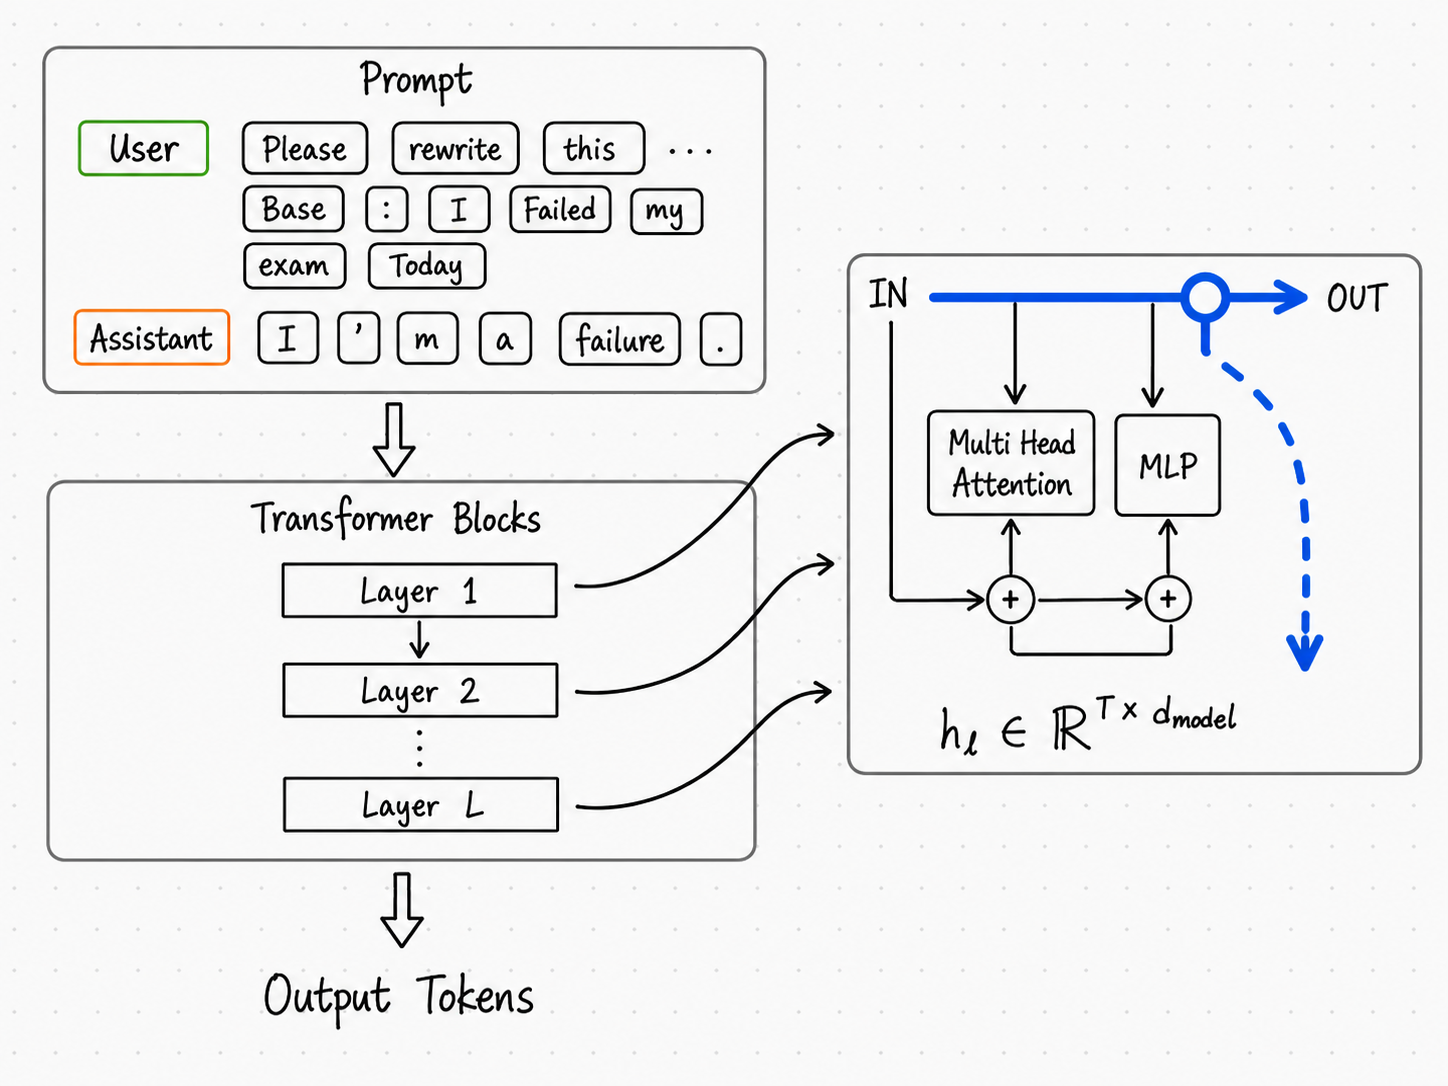
\includegraphics[width=0.6\linewidth]{figures/residual_extraction.png}
    \caption{Schematic overview of residual stream extraction during a forward pass. Tokenisation process is simplified for clarity. In reality, the input is tokenised into subword units e.g. ``please'' might be tokenised into ``ple'' and ``ase''.}
    \label{fig:residual_extraction}
\end{figure}

For each target layer $l$, the last token's hidden state is taken from the layer's output, i.e.
\[
\mathbf{h}_{l}=\texttt{hidden\_states}[l+1][:,-1,:]
\] 
Since tokenisation uses left padding, the index $-1$ consistently corresponds to the \textbf{final} real token in each sequence in the batch. Final-token representation is the state after the model has processed the entire rewritten utterance, making it a compact summary of the affective framing expressed by the continuation. Activations are sampled from layers $\{8,10,13,16,19,22\}$, producing a multi-layer representation for every input.

In summary, the emotion-intensity extraction pipeline produces a 5D tensor:
\[
\mathbf{H}^{\text{emo}} \in \mathbb{R}^{N \times E \times I \times L \times D},
\]
where $N$ is the number of source texts, $E=8$ emotions rewrites, $I=3$ intensity levels, $L$ is the number of sampled layers, and $D=4096$ is the hidden dimension. The neutral baseline pipeline produces:
\[
\mathbf{H}^{\text{neu}} \in \mathbb{R}^{N \times L \times D}.
\]
Source IDs are sorted to align both tensors by index, allowing direct subtraction
\[
\Delta\mathbf{H}_{n,e,i,l,:}=\mathbf{H}^{\text{emo}}_{n,e,i,l,:}-\mathbf{H}^{\text{neu}}_{n,l,:},
\]
which isolates affective shifts while controlling for base semantic content.

\section{Layer Selection and Diagnostics}
\label{sec:layer_selection}

Not all transformer layers provide equally useful representations for affective analysis. Emotion-related structure may be present at multiple depths, but different layers can privilege different properties of the representation. As described in the Roadmap~\ref{steering_roadmap_1}, the aim of the layer selection stage is to identify the layer where emotion before verbalisation are best abstracted. For example, one layer may provide strong emotion-category separability, while another may better preserve a compact low-dimensional geometry. We define three diagnostic metrics to evaluate candidate layers:

\begin{enumerate}
  \item \textbf{Balanced Accuracy}: This metric measures if that layer preserves the emotion category information. We train a logistic regression model to predict the emotion category from the residual vectors, which are PCA-ed into a 4D subspace. The higher this value is, the more our residual space possesses a structure that can be linearly mapped to human-named emotion labels.
  \item \textbf{Geometric Compactness}: This shows if the emotion information is concentrated in a low-dimensional subspace. We measure the explained variance ratio (EVR) of the emotion centroids in the residual space. This metric assesses to what extent the few principal components extracted by PCA/SVD can explain the variance in the original residual vector set.
  \item \textbf{Graded Affect Sensitivity}: This metric quantifies whether the representation of that layer merely ``separates emotion categories'' or whether it possesses ``emotional quantity, and intensity'' as continuous variables. By performing PCA for each emotion label and projecting all samples onto the vector with the greatest variance within each emotion (PC1), we obtain coordinates indicating the position of each sample on the PC1 axis. The Spearman correlation between this score and the intensity label (low, medium, high) serves as a measure indicating that the vector of greatest variation within that emotion aligns with the intensity level. This is then averaged across the eight emotions.
\end{enumerate}

\begin{table}[H]
\centering
\small
\begin{tabular}{lccc}
\toprule
\textbf{Layer} &
  \textbf{Balanced Acc} &
  \textbf{EVR\textsubscript{4}} &
  \textbf{Graded Affect Sensitivity} \\
  & \textit{(4-D subspace)} & & \\
\midrule
  8  & 0.6914 & 0.8834 & 0.1312 \\
  10 & 0.6751 & 0.8876 & 0.0998 \\
  13 \textbf{*} & \textbf{0.7033} & 0.8920 & \textbf{0.1336} \\
  16 & 0.6704 & \textbf{0.8958} & 0.1297 \\
  19 & 0.6198 & 0.8902 & 0.1142 \\
  22 & 0.6142 & 0.8928 & 0.1022 \\
\bottomrule
\end{tabular}
\caption{Layer-wise diagnostic summary for candidate layers. Emotion-category probe balanced accuracy (4-D subspace), centroid compactness (EVR\textsubscript{4}), and mean local intensity-vector correlation. Bold indicates the best value per column; asterisk marks the selected reporting layer.}
\label{tab:layer_diagnostics}
\end{table}

Based on these diagnostics, layer 13 was selected as the primary layer for the main analyses. It is not globally best on every metric, but it provides the most convincing overall trade-off between the above three criteria.

\begin{figure}[H]
    \centering
    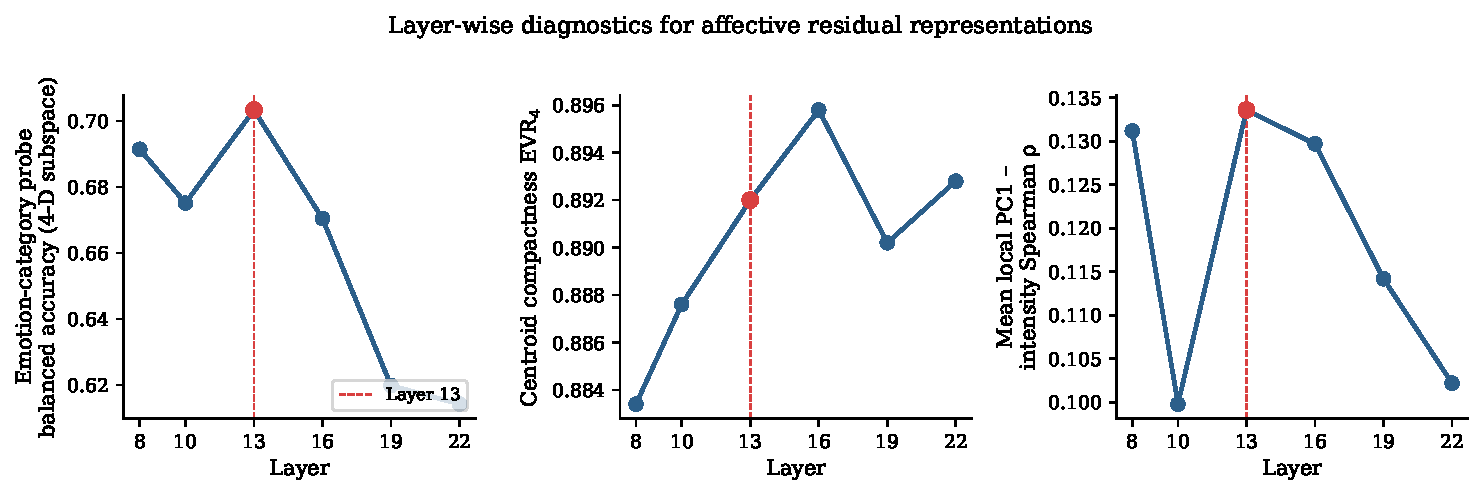
\includegraphics[width=0.8\linewidth]{figures/layer_diagnostics_lineplot.pdf}
    \caption{A visualisation of the layer diagnostics across candidate layers.}
    \label{fig:layer_diagnostics}
\end{figure}

Firstly, \textbf{layer 13 achieves the highest balanced accuracy of all the candidate layers}. Balanced accuracy reaches $0.7033$ in the residual subspace, compared to $0.6914$ in layer 8, $0.6751$ in layer 10 and $0.6704$ in layer 16. This suggests that the emotional representation in layer 13 can be most easily converted into human-named emotion categories, even after compression into a small number of dimensions. However, this does not necessarily mean that the model represents emotions as discrete symbolic labels. Rather, it indicates that the continuous affective geometry at this layer is organised in such a way that human emotion categories can be identified using a simple linear classifier.\par

Secondly, \textbf{layer 13 preserves a highly compact, low-dimensional geometry}. Its centroid-level $\mathrm{EVR}_{4}$ is $0.8920$, meaning that the top four principal components explain $89.2\%$ of the variance among the emotion centroids. Although layer 16 has the highest $\mathrm{EVR}_{4}$ value ($0.8958$), the difference between layers 13 and 16 is small. Therefore, the stronger category decodability at layer 13 does not appear to result in a loss of the low-dimensional affective structure. In this sense, layer 13 preserves a geometry that is both compact and interpretable.\par

Thirdly, \textbf{layer 13 shows the highest graded affect sensitivity of all the tested layers}. The mean intensity-vector correlation is $0.1336$ at layer 13, compared to $0.1312$ at layer 8, $0.0998$ at layer 10 and $0.1297$ at layer 16. As the absolute value is modest, we do not interpret the local PC1 of each emotion as a pure intensity axis. Instead, this metric should be interpreted as an indication of whether the dominant variation within each emotion retains some monotonic relationship with affective strength. The fact that layer 13 achieves the highest value suggests that it preserves slightly more graded affective information than neighbouring layers.\par

Taken together, these diagnostics suggest that layer 13 is close to a useful abstraction point for pre-verbal affective structures. Earlier layers, such as layers 8 and 10, retain substantial affective information, but their category recoverability and graded sensitivity are weaker or less stable. Later layers, such as layer 16, have a marginally more compact geometry but show lower emotion-category balanced accuracy. This indicates that later representations are shaped by subsequent verbalisation. Therefore, layer 13 offers the best overall trade-off: it is low-dimensional enough to support geometric analysis and linearly organised enough to recover human emotion labels. It is also sensitive enough to retain graded affective variation.\par

We therefore use layer 13 as the primary reporting layer in subsequent analyses. However, we do not treat it as the only layer at which affective structure exists. Neighbouring layers show similar trends, indicating that the affective geometry is distributed across multiple middle layers rather than being localised to a single transformer block. Layer 13 should be understood as the most suitable operational layer for this study, i.e. the layer at which the representation is most useful for modelling emotion before it is collapsed into explicit verbal labels.\par

\section{CAA Vector Construction}
\label{sec:caa_construction}

\begin{figure}[H]
    \centering
    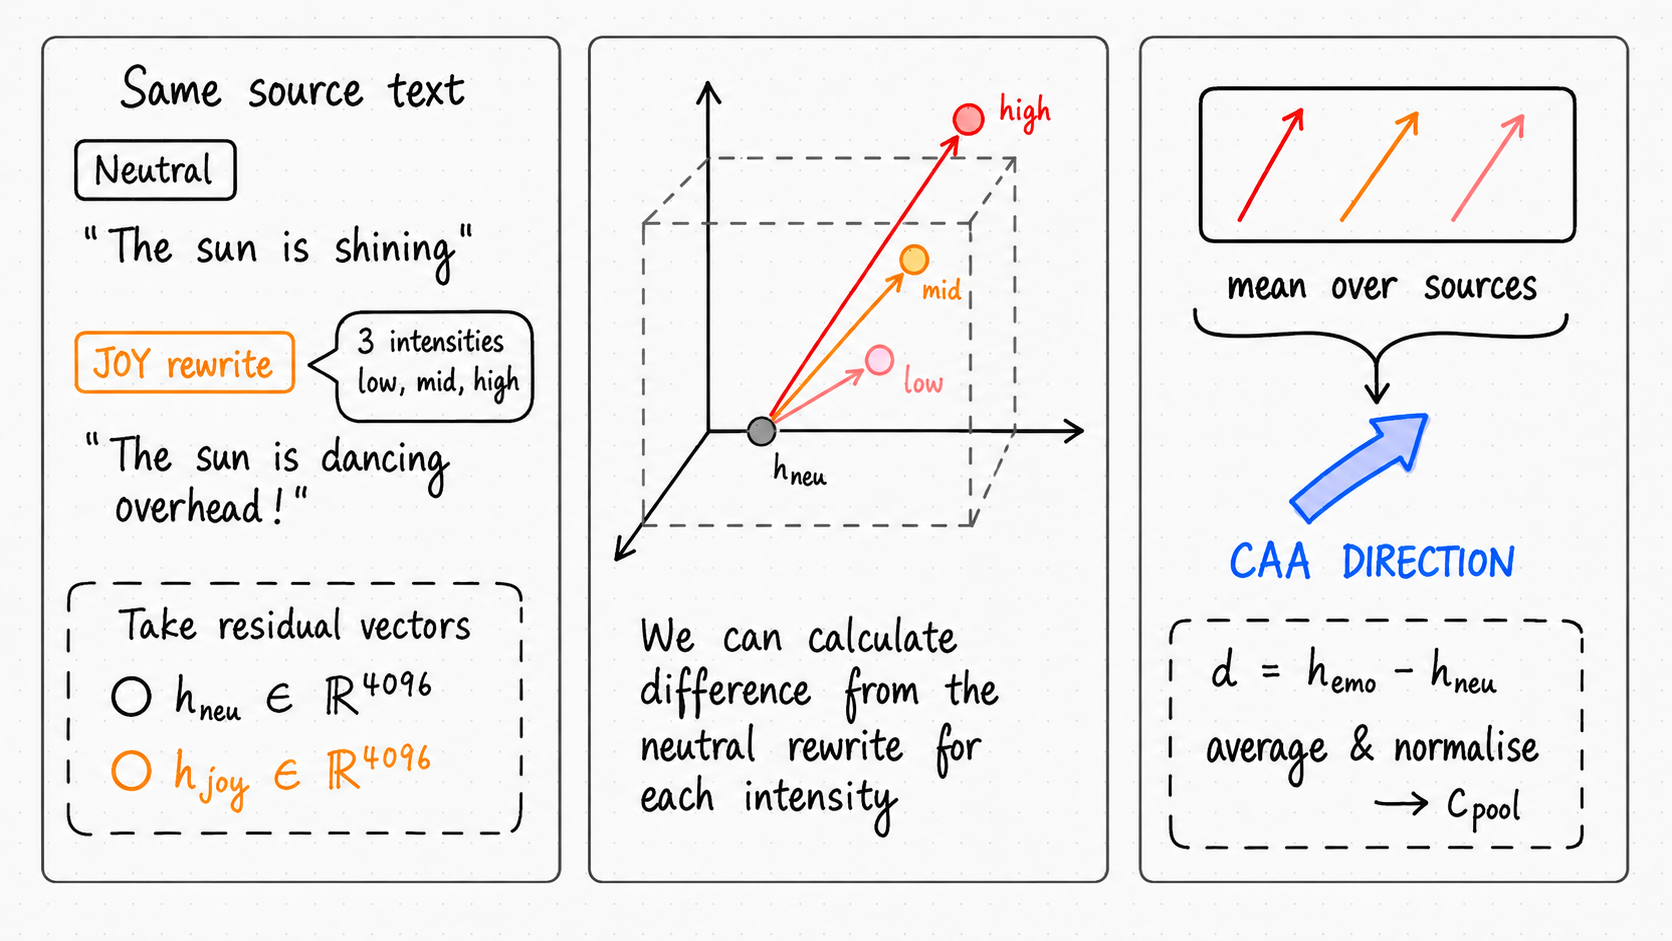
\includegraphics[width=0.6\linewidth]{figures/caa_construction.png}
    \caption{Schematic overview of CAA vector construction.}
    \label{fig:caa_construction}
\end{figure}

In order to convert contrastive residual differences into controllable steering signals, we derive Contrastive Activation Addition (CAA) vectors from emotional and neutral conditioned activations. For each source utterance $n$, emotion $e$, intensity level $i$, and layer $l=13$, we first define
\[
\Delta_{n,e,i,l}=\mathbf{h}^{\mathrm{emo}}_{n,e,i,l}-\mathbf{h}^{\mathrm{neu}}_{n,l}.
\]
We then average over sources and normalise to unit length:
\[
\bar{\Delta}_{e,i,l}=\frac{1}{N}\sum_{n=1}^{N}\Delta_{n,e,i,l},
\qquad
\mathbf{c}_{e,i,l}=\frac{\bar{\Delta}_{e,i,l}}{\lVert\bar{\Delta}_{e,i,l}\rVert_2}.
\]
The vectors $\mathbf{c}_{e,i,l}$ are intensity-specific CAA vectors.

As the steering stage primarily targets the emotional category, treating intensity as a secondary modulation, we also build \textbf{mean emotion vector} $\mathbf{c}^{\mathrm{pool}}_{e,l}$ by averaging across intensities and re-normalising:
\[
\mathbf{c}^{\mathrm{pool}}_{e,l}
=
\frac{\frac{1}{I}\sum_{i=1}^{I}\bar{\Delta}_{e,i,l}}
{\left\lVert\frac{1}{I}\sum_{i=1}^{I}\bar{\Delta}_{e,i,l}\right\rVert_2}.
\]

In the main steering analyses, these pooled unit vectors are used as the primary candidate steering vectors. \par

Figure~\ref{fig:caa_construction} illustrates the construction process. For each emotion and intensity, we compute the mean contrastive shift across sources, and then normalise to obtain a unit vector. The pooled vector is obtained by averaging the intensity-specific vectors and re-normalising. This process yields a set of emotion-specific CAA vectors that can be used for steering interventions.\par

We first confirm that the construction is stable: at layer 13, mean cosine similarity between per-source contrastive shifts $\Delta_{n,e} = h^\text{emo}_{n,e} - h^\text{neu}_n$ and the global CAA vectors $\mathbf{c}^\text{pool}_{e,13}$ ranges from $0.8536$ to $0.8570$ (standard deviation $\approx 0.054$), confirming that the averaged vector is representative rather than an artefact of a few extreme samples.\par

However, inspecting the directions across emotion categories reveals a striking pattern. To preserve the source-pairing structure inherent in the dataset, we compute inter-emotion similarity per source text and then average: for each pair $(e_1, e_2)$, we report $\frac{1}{N}\sum_n \cos(\hat{\Delta}_{n,e_1},\,\hat{\Delta}_{n,e_2})$, where $\hat{\Delta}_{n,e}$ is the unit-normalised per-source shift pooled over intensities. The diagonal shows within-emotion intensity consistency: the mean per-source cosine across low, medium, and high intensity shifts of the same emotion. The resulting matrix is shown in Figure~\ref{fig:caa_paired_inter_emotion_cosine_heatmap_L13}.\par

\begin{figure}[H]
  \centering
  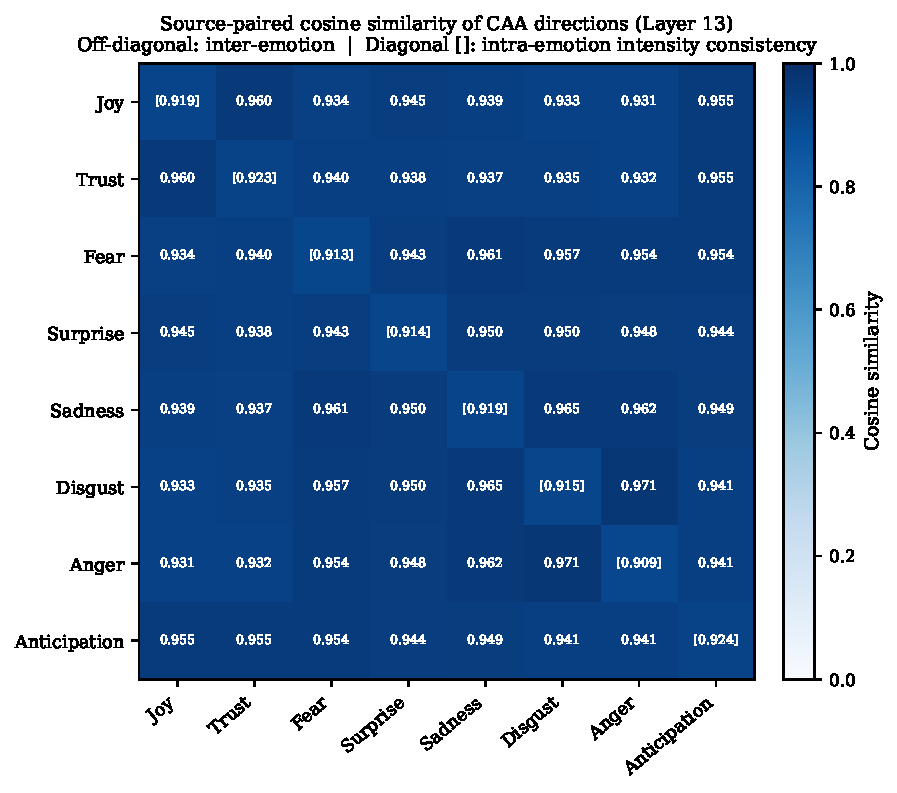
\includegraphics[width=0.75\linewidth]{figures/caa_paired_inter_emotion_cosine_heatmap_L13.pdf}
  \caption{Source-paired cosine similarity of CAA directions at layer 13. Off-diagonal: mean per-source cosine between emotion pairs. Diagonal \texttt{[\,]}: within-emotion intensity consistency (mean per-source cosine across low/medium/high intensity pairs). Colour scale spans $[0, 1]$; all entries lie above $0.90$.}
  \label{fig:caa_paired_inter_emotion_cosine_heatmap_L13}
\end{figure}

All values lie in the range $0.91$--$0.97$. More strikingly, for several emotion pairs such as \textit{disgust}--\textit{anger} ($0.971$) and \textit{sadness}--\textit{disgust} ($0.965$), the inter-emotion similarity \textbf{exceeds} the within-emotion intensity consistency shown on the diagonal ($0.91$--$0.92$). This means that for the same source text, the shift toward \textit{disgust} is more similar to the shift toward \textit{anger} than the low-intensity \textit{disgust} shift is to the high-intensity \textit{disgust} shift.\par

This uniformity would be unexpected if each CAA vector primarily encoded emotion-specific information. Instead, it suggests that \textbf{all vectors are dominated by a shared emotionalisation component}. This common axis is activated regardless of the targeted emotion. \par

The model appears to shift representations in two stages. First, it shifts from a neutral sentence to a generic emotional sentence. Then, from that shared emotional context, it moves towards a particular affective category. A raw CAA vector conflates both stages. This makes the emotion-specific signal difficult to access directly. This observation motivates the explicit decomposition introduced in the next section.\par

\section{Decomposition}
\label{sec:decomposition}

The pooled CAA vectors at layer 13 are highly aligned across emotion categories, suggesting that each vector contains a large shared component corresponding to generic emotionalisation. To separate this common shift from emotion identity, we define a shared vector as the normalised mean over emotion-specific pooled CAA vectors:
\[
\mathbf{g}=
\frac{\frac{1}{|E|}\sum_{e\in E}\mathbf{c}^{\mathrm{pool}}_{e,13}}
{\left\lVert\frac{1}{|E|}\sum_{e\in E}\mathbf{c}^{\mathrm{pool}}_{e,13}\right\rVert_2}.
\]
We then remove this shared component from each pooled vector by orthogonal projection:
\[
\mathbf{r}_e=\mathbf{c}^{\mathrm{pool}}_{e,13}-\left((\mathbf{c}^{\mathrm{pool}}_{e,13})^\top \mathbf{g}\right)\mathbf{g}.
\]
For steering, we use the unit-normalised residual
\[
\hat{\mathbf{r}}_e=\frac{\mathbf{r}_e}{\lVert\mathbf{r}_e\rVert_2},
\]
and construct interventions as
\[
\Delta_e(\alpha_G,\alpha_R)=\alpha_G\mathbf{g}+\alpha_R\hat{\mathbf{r}}_e.
\]

In this chapter, we treat this decomposition as an operational parameterisation for controllable steering: $\mathbf{g}$ controls global emotionalisation strength, while $\hat{\mathbf{r}}_e$ controls emotion-specific directionality. It is based on the same linear intervention assumption that underlies CAA. Behavioural features can be represented approximately as directions in the residual stream, and adding a vector in such a direction can modulate the corresponding behaviour causally. Assuming this, if emotion-specific CAA vectors are strongly aligned, their shared direction naturally estimates the component common to emotional responses across categories. \par

The mean direction, represented by the vector $\mathbf{g}$, captures the component that is consistently present across emotion categories. Since category-specific components are expected to vary with $e$, averaging over emotions should reduce idiosyncratic, identity-related components while preserving the common direction across all emotionalised generations. We therefore interpret $\mathbf{g}$ as an estimate of generic emotionalisation, i.e. a direction that increases the overall emotional character of the output independently of any particular emotion label. \par

The residual vector \(\mathbf{r}_e\) is obtained by subtracting the orthogonal projection of \(\mathbf{c}^{\mathrm{pool}}_{e,13}\) onto \(\mathbf{g}\), which removes the part of the emotion-specific CAA vector explained by the shared emotionalisation direction. Consequently, \(\mathbf{r}_e\) satisfies \(\mathbf{r}_e^\top \mathbf{g}=0\), meaning that, to first order in the linear residual-stream approximation, changes along \(\hat{\mathbf{r}}_e\) do not directly change the generic emotionalisation coordinate. The residual therefore isolates the remaining category-specific variation: the part of the vector that distinguishes one emotion from the shared emotional shift. \par

Further unit-normalising \(\mathbf{r}_e\) separates direction from intervention strength. The residual norm may depend on the size of the dataset, the variance within categories, the pooling choices made, or the strength with which a particular emotion is represented at layer 13. Using the normalised residual vector, the coefficient \(\alpha_R\) has a comparable interpretation across emotions: it controls how far the activation is moved in the category-specific residual direction rather than inheriting arbitrary differences in residual vector magnitude.\par

The final intervention
\[
\Delta_e(\alpha_G,\alpha_R)=\alpha_G\mathbf{g}+\alpha_R\hat{\mathbf{r}}_e
\]
therefore provides two independently interpretable steering controls. The coefficient \(\alpha_G\) modulates the shared emotionalisation component, while \(\alpha_R\) modulates the emotion-specific residual component. This makes it possible to test whether emotional intensity and emotion identity can be controlled separately: increasing \(\alpha_G\) should primarily increase the degree of emotionalisation, whereas increasing \(\alpha_R\) should primarily increase the recognisability of the target emotion.\par

This procedure should not be understood as recovering a single, accurate decomposition of emotional representations. Rather, it is a deliberately constrained linear decomposition, driven by the high degree of alignment observed among pooled emotion CAA vectors. The resulting two-parameter interventions are assessed for their empirical validity based on whether they exhibit the intended behavioural dissociation between generic emotionalisation and emotion-specific identity.\par

\begin{figure}[H]
    \centering
    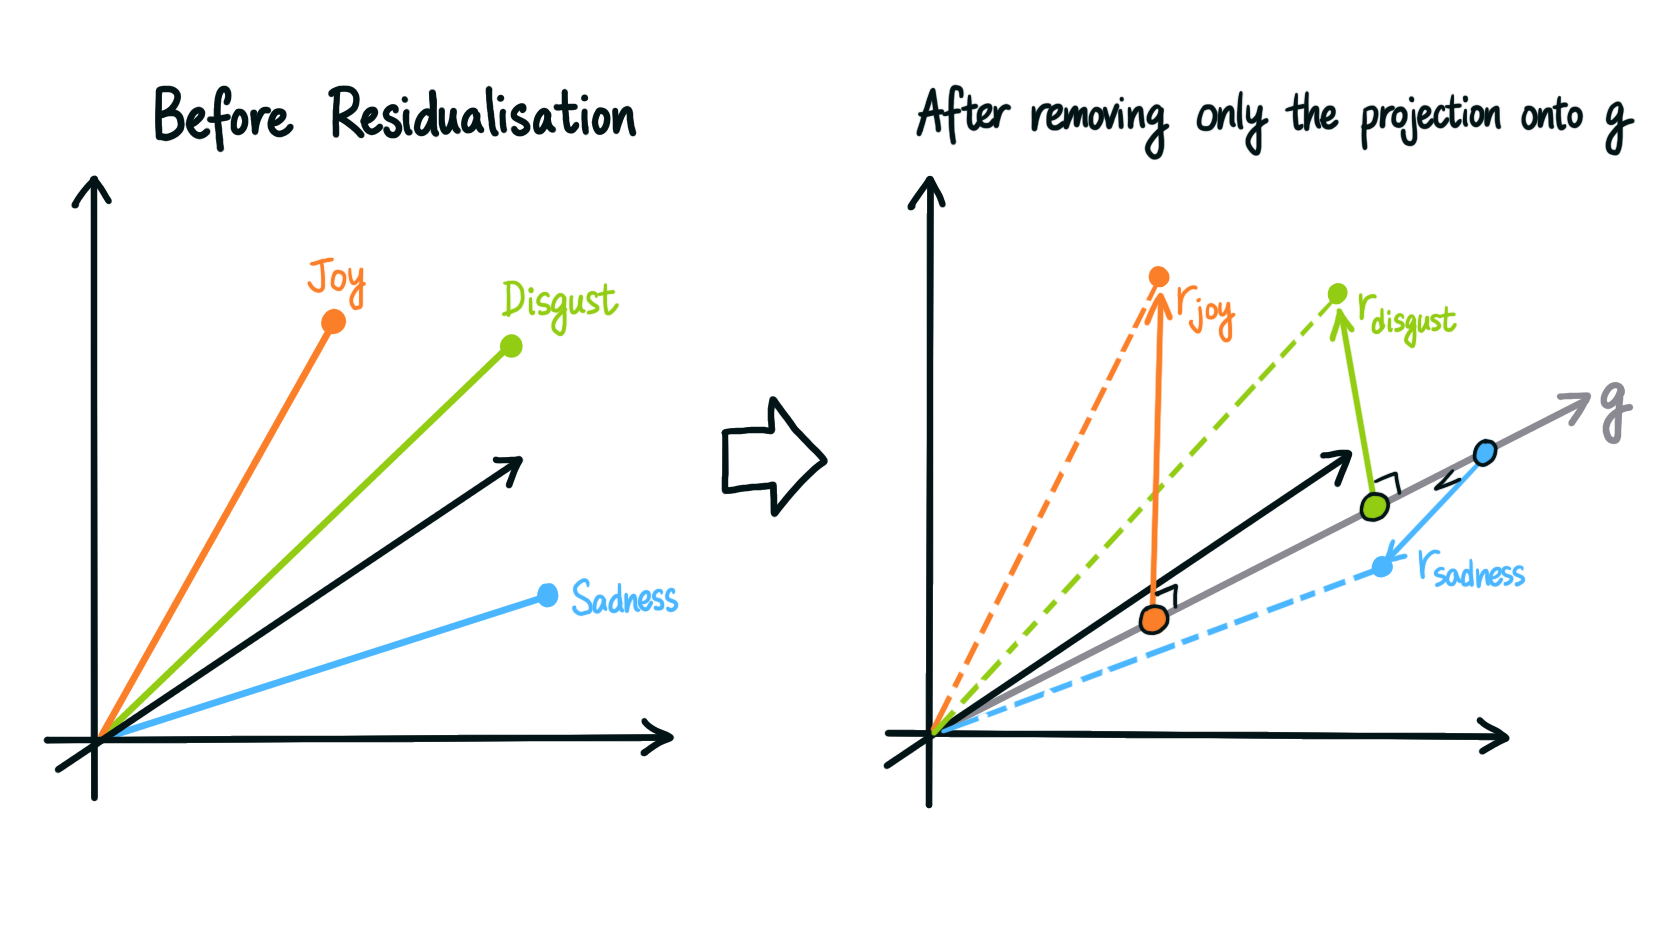
\includegraphics[width=0.8\linewidth]{figures/g_residualisation.png}
    \caption{Operational decomposition of emotion CAA vectors into a shared emotionalisation component $g$ and an emotion-specific residual component $\hat{r}_e$. The left panel shows the original CAA vectors for three example emotions (joy, disgust and sadness). The right panel shows the same vectors after removing the shared component $g$, revealing the residual vectors $\hat{r}_e$ that are specific to each emotion.}
    \label{fig:g_residualisation}
\end{figure}

\section{Decomposition Validity}
\label{sec:decomposition_validity}
%TODO

\section{Steering Experiments}
\label{sec:steering_experiments}

\subsection{Generation Setup}

We investigate whether emotion-specific residuals $\hat{\mathbf{r}}_e$ causally bias text generation towards the target emotion, and specifically, whether incorporating the shared vector $\mathbf{g}$ at any scale yields further benefits. We generate follow-up sentences using \texttt{Llama-3.1-8B-Instruct} from 100 source utterances sampled from the test split of the emotion rewriting dataset. To eliminate sampling variance as a confounding factor, we employ greedy decoding (temperature $= 0$) throughout the entire process.

\subsubsection*{Sweep Design}

Based on preliminary exploration, we fix $\alpha_R = 5.0$ as the residual scale that demonstrated the best performance, and scan $\alpha_G \in \{0, 0.25, 0.5, 1, 2, 3\}$. The anchor condition $\alpha_G = 0$ corresponds to pure residual steering (i.e. no shared components). The introduction of fine intermediate values ($0.25$, $0.5$, $1$, $2$) was intended to verify whether contributions from $\mathbf{g}$ below a certain threshold are beneficial before the scaling becomes detrimental. Each combination of source text, target emotion, and $\alpha_G$ value constitutes a single generation, resulting in a total of $100 \times 8 \times 6 = 4,800$ generated texts.


\subsection{Automated Evaluation Protocol}

Each generated sentence is scored by \texttt{gpt-4o-mini}, which acts as a judge. To ensure consistent evaluation criteria across all $4800$ items, the judge is presented with three fixed few-shot examples that cover the entire scoring range. Specifically, these are examples that match a high-quality target, examples where the meaning is preserved but the emotion expressed is incorrect, and examples where the target emotion is partially present but the propositional content is off-target. These examples serve to anchor the two endpoints of the evaluation scale before the evaluator views the test items. Scores are retrieved via OpenAI's Structured Output API, which utilises a strict JSON schema. This eliminates the need for free-form parsing and ensures that the three numerical scores and the dominant sentiment label are always returned in a consistent, machine-readable format. The evaluators operate without being informed of the intervention condition (the $\alpha_G$ value).

Three continuous $[0,1]$ metrics are collected per item:

\begin{itemize}
  \item \textbf{Target-emotion match}: Whether the predominant emotional tone of the output matches the target emotion. The judge is shown the target emotion label and asked to rate the degree to which the generated text conveys that emotion as its primary sentiment.
  \item \textbf{Semantic preservation}: Whether the core propositional content of the source utterance is retained. The judge compares the generated text with the original to assess whether the same events, entities, and relationships are present.
  \item \textbf{Emotionality}: Whether the output contains any emotional expression at all. A low score flags outputs that are flat, incoherent, or affectively empty, serving as a quality check: an intervention that appears to improve target-emotion match by producing incoherent text will be exposed by a corresponding drop on this metric.
\end{itemize}

\subsection{Statistical Analysis}

The mean values for each condition are reported together with the 95\% confidence intervals calculated from the score distributions for each item. To verify whether an arbitrary $\alpha_G > 0$ reliably exceeds the anchor value of $\alpha_G = 0$, items are paired using the key $({\rm source\_id},\,{\rm target\_emotion})$ for target emotion agreement, and a paired $t$-test is applied. By performing the pairing within this key, we control for sentence-level and emotion-level variations common to all $\alpha_G$ conditions, obtaining $n = 800$ pairs per test whilst achieving confidence intervals that are significantly narrower than those obtained in non-paired comparisons.

\subsection{Results}
\label{sec:alpha_g_sweep}

We hold $\alpha_R = 5.0$ fixed and sweep $\alpha_G \in \{0, 0.25, 0.5, 1, 2, 3\}$ across $n = 800$ samples per condition ($100$ source texts $\times$ $8$ target emotions). This directly answers whether adding $\mathbf{g}$ helps at any scale.

Figure~\ref{fig:alpha_g_sweep_aggregate} shows all three metrics as a function of $\alpha_G$. All three decline monotonically as $\alpha_G$ increases. Target-emotion match falls from $0.270$ at $\alpha_G = 0$ to $0.252$ at $\alpha_G = 3$; emotionality drops from $0.567$ to $0.531$; and semantic preservation declines from $0.870$ to $0.863$. No value of $\alpha_G > 0$ produces any reliable improvement over $\alpha_G = 0$ on any metric. The per-emotion breakdown (Figure~\ref{fig:alpha_g_sweep_per_emotion}) confirms that no individual emotion benefits from a positive $\alpha_G$.

\begin{figure}[H]
\centering
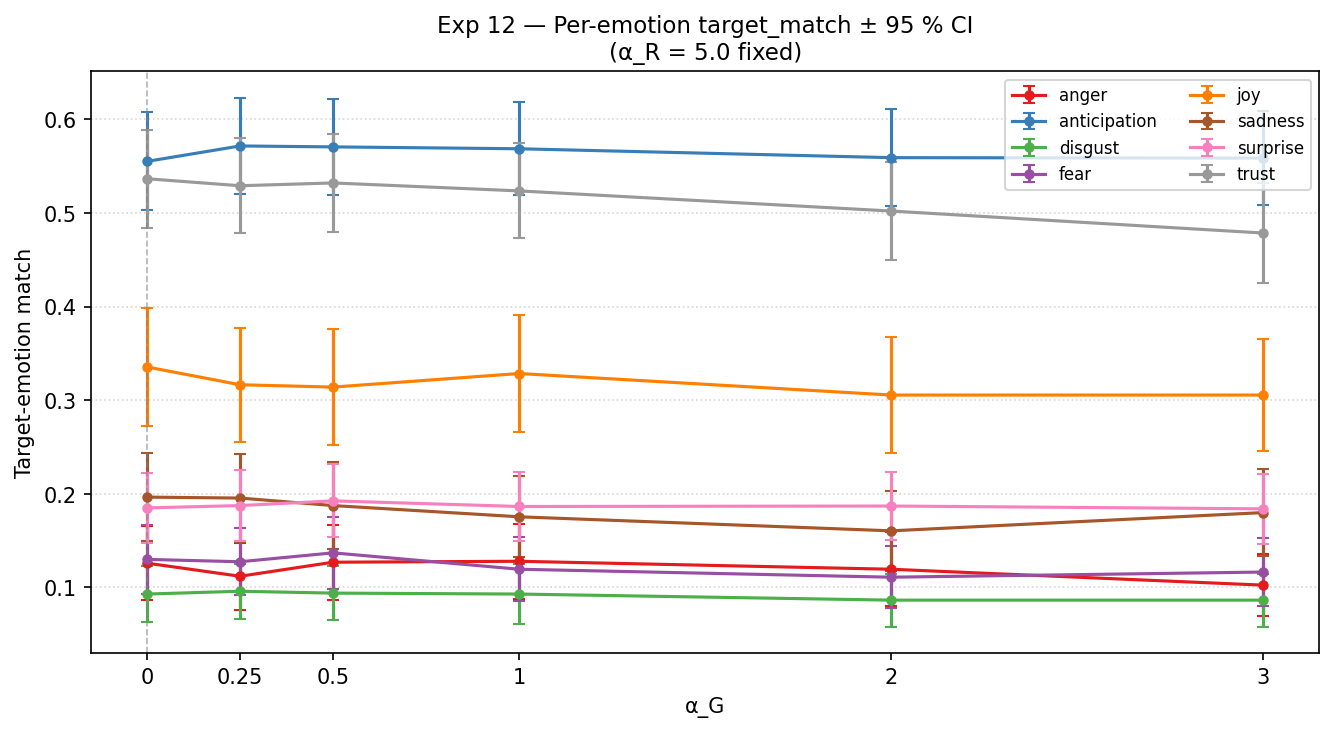
\includegraphics[width=\linewidth]{figures/alpha_g_sweep_per_emotion.png}
\caption{Per-emotion target-emotion match vs.\ $\alpha_G$ ($\alpha_R = 5.0$ fixed; $n = 100$ per cell; error bars = 95\% CI). No individual emotion benefits from a positive $\alpha_G$.}\label{fig:alpha_g_sweep_per_emotion}
\end{figure}

\begin{figure}[H]
\centering
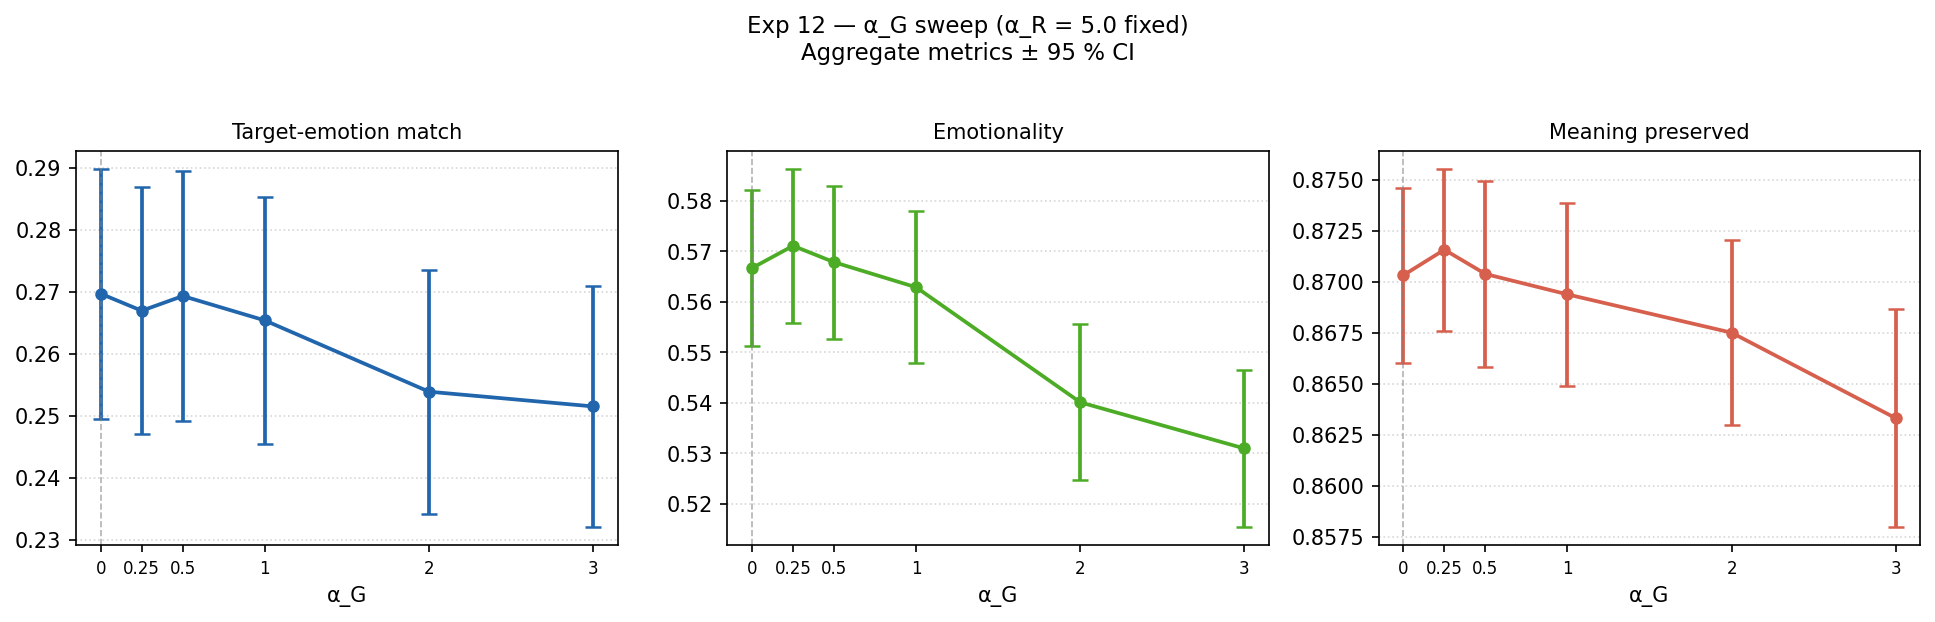
\includegraphics[width=\linewidth]{figures/alpha_g_sweep_aggregate.png}
\caption{Target-emotion match, emotionality, and semantic preservation as a function of $\alpha_G$, with $\alpha_R = 5.0$ fixed ($n = 800$ per condition; error bars = 95\% CI). All three metrics decrease monotonically as $\alpha_G$ increases from $0$.}\label{fig:alpha_g_sweep_aggregate}
\end{figure}

The shared direction $\mathbf{g}$ is counterproductive at every tested scale. Effective affective steering therefore reduces to $\Delta_e = \alpha_R\,\hat{\mathbf{r}}_e$, with $\alpha_G$ discarded.

\section{Causal Validation: Steering}
\label{sec:steering_causal_validation}

To confirm that the emotion-specific residual $\hat{\mathbf{r}}_e$ provides a reliable steering signal, we perform a generation experiment using pure residual steering ($\alpha_G = 0$, $\alpha_R = 5.0$). This tests whether adding $\hat{\mathbf{r}}_e$ alone can bias generation towards the target emotion, and whether the resulting outputs exhibit the expected pattern of emotional shift without excessive loss of semantic content.

\subsection{Activation Hook}
The steering intervention is implemented as a forward hook registered in the layer 13 of the transformer. In each forward pass, this hook captures the hidden state $\mathbf{h} \in \mathbb{R}^{B \times T \times D}$ of the residual stream generated by that layer, and adds $\Delta_e$ only to the slice of the final token:
\[
\mathbf{h}_{:,\,-1,\,:} \;\leftarrow\; \mathbf{h}_{:,\,-1,\,:} + \Delta_e(\alpha_G, \alpha_R),
\]
where $\Delta_e = \alpha_G\,\mathbf{g} + \alpha_R\,\hat{\mathbf{r}}_e$. By applying the perturbation only to the final prompt token, we concentrate the causal signal at the point where the model begins its autoregressive generation, whilst keeping the contextual representations of all preceding tokens unchanged. To prevent interference between invocations, the hook is released immediately after generation is complete.

\subsection{Result}

Table~\ref{tab:qualitative_steering_examples} shows representative examples of residual-only steering ($\alpha_G = 0$, $\alpha_R = 5$, last-token intervention at layer 13). The intervention does not simply overwrite the source context; instead, it bends the existing situation toward the target affective framing.

\begin{table}[H]
\centering
\small
\begin{tabular}{p{0.13\linewidth} p{0.13\linewidth} p{0.30\linewidth} p{0.34\linewidth}}
\toprule
\textbf{Seed} & \textbf{Target} & \textbf{Seed utterance} & \textbf{Steered output} \\
\midrule
fear & joy &
Walking alone through the dark alley I felt a cold shiver run down my spine. &
As I strolled through the dimly lit alley, the flickering streetlights cast a warm glow, but the sense of solitude and tranquility that filled the air made me feel a gentle, soothing calm wash over me. \\
\midrule
disgust & joy &
The smell from the bin was overwhelming and the sight of it made my stomach turn. &
The putrid aroma wafting from the trash can was a welcome respite, and the vibrant colors of the discarded items made my heart feel uplifted. \\
\bottomrule
\end{tabular}
\caption{Representative examples of residual-only CAA steering ($\alpha_G = 0$, $\alpha_R = 5$). The fear-to-joy example shows a natural affective shift while preserving the dark-alley context. The disgust-to-joy example shows a more extreme reinterpretation, illustrating both the causal reach and the contextual limits of the intervention.}
\label{tab:qualitative_steering_examples}
\end{table}

Both examples illustrate the same pattern: the residual intervention shifts the emotional framing without replacing the underlying situation. The fear-to-joy output preserves the alley but reframes it as tranquil; the disgust-to-joy output retains the bin but reinterprets its contents positively. The final output remains bounded by the semantic content of the source, consistent with the modest but consistent target-emotion match gains seen in the quantitative results.

\subsection{Interpretation}

The $\alpha_G$ sweep gives a clear answer: adding the shared emotionalisation direction $\mathbf{g}$ hurts performance at every tested scale. All three evaluation metrics decline monotonically as $\alpha_G$ increases, and this holds for all eight target emotions without exception. The practical conclusion is that the two-component formula $\Delta_e = \alpha_G\,\mathbf{g} + \alpha_R\,\hat{\mathbf{r}}_e$ reduces in practice to its residual term alone: $\Delta_e = \alpha_R\,\hat{\mathbf{r}}_e$.\par

This finding also clarifies what the decomposition achieves. The pooled CAA vector $\mathbf{c}^{\mathrm{pool}}_e$ is dominated by $\mathbf{g}$ (as the high cross-emotion cosine similarities in Section~\ref{sec:caa_construction} showed), so steering with the raw pooled vector is largely equivalent to adding $\mathbf{g}$~--and therefore counterproductive. The decomposition separates $\mathbf{g}$ from $\hat{\mathbf{r}}_e$ precisely so that the useful component can be used in isolation. The steering effect is modest rather than absolute: the intervention biases the output toward the target emotion while remaining constrained by the initial utterance, and larger $\alpha_R$ provides only partial directional control. These limitations motivate the structural analysis of $\hat{\mathbf{r}}_e$ in the next chapter.\par

\section{Limitations and Transition}

These results confirm that affective steering can be implemented as a decomposed residual-space intervention, and that the effective operating point is $\alpha_G = 0$, $\alpha_R > 0$. The shared direction $\mathbf{g}$ is counterproductive at every tested scale; only the emotion-specific residual $\hat{\mathbf{r}}_e$ provides a reliable steering signal. This conclusion was only reachable because the decomposition made the two components separable and independently testable.\par

However, the results also reveal two limitations. First, the steering effect is modest rather than absolute: target-emotion match improves consistently but remains well below ceiling, and the intervention is bounded by the semantic and emotional content of the source utterance. Second, the effect magnitude varies substantially across emotions, suggesting that the discriminative power of $\hat{\mathbf{r}}_e$ differs by emotion category — a structural question addressed in the next chapter.\par

These limitations motivate the next chapter. So far, $\hat{\mathbf{r}}_e$ has been treated as a single entity. The next chapter asks what this residual actually represents. In particular, it examines whether emotions such as joy, sadness, and anger should be treated as atomic vectors, or whether they contain local sub-axes that correspond to more subtle, pre-verbal affective vectors.